\documentclass[twocolumn]{article}

\usepackage{geometry}
\geometry{textwidth = 18cm,textheight = 24cm}

\usepackage{cite}
\usepackage{caption}
\usepackage{graphicx}
\usepackage{amsmath}
\usepackage{amssymb}
%\usepackage{braket}
\usepackage{textcomp}
%\usepackage{lmodern}
\usepackage{authblk}
\usepackage{datetime}
\usepackage{gensymb}
\usepackage{wrapfig}
%\usepackage[usenames,dvipsnames,svgnames,table]{xcolor}
\usepackage{booktabs}
%\usepackage{appendix}

%\usepackage[switch,columnwise]{lineno}
%\linenumbers

\newcommand{\onlinecite}[1]{\hspace{-1 ex} \nocite{#1}\citenum{#1}} 

\let\OLDthebibliography\thebibliography
\renewcommand\thebibliography[1]{
  \OLDthebibliography{#1}
  \setlength{\parskip}{0pt}
  \setlength{\itemsep}{0pt plus 0.3ex}
}
  
\title{Modeling Loop Neurons as Systems of Coupled Leaky Integrators}
\author[1]{\Large{NIST Physics and Hardware for Intelligence Project}
\\
\textit{\large{National Institute of Standards and Technology}}
\\
\vspace{-0.2em}
\textit{\large{325 Broadway, Boulder, CO, USA, 80305}}
\\
\vspace{-0.2em}
\textit{\large{jeffrey.shainline@nist.gov}}
}
\date{\today}%\today

\begin{document}

\twocolumn[
  \begin{@twocolumnfalse}
    \maketitle
    \begin{abstract}

Superconducting optoelectronic loop neurons are a class of circuits potentially conducive to realizing networks for large-scale artificial cognition. These circuits employ superconducting components including single-photon detectors, Josephson junctions, and transformers. To date, all simulations of loop neurons have used first-principles circuit analysis to model the behavior of synapses, dendrites, and neurons. These circuit models are computationally inefficient and leave opaque the relationship between loop neurons and other neuron models employed in computational neuroscience and cognitive computing. Here we introduce a modeling framework that captures the behavior of the relevant synaptic, dendritic, and neuronal circuits at a phenomenological level without resorting to full solutions to the circuit equations. In this framework, each synapse and dendrite is discovered to obey a single leaky-integrator ordinary differential equation, while a neuron with adaptive refraction is modeled as two dendrites in a feedback configuration. We quantify the accuracy of the phenomenological model relative to circuit simulations, and find that the approach not only reduces the total number of differential equations in the coupled system, but also allows an increase in the numerical time step by a factor of 100. We demonstrate the use of the model with several basic examples. The net increase in computational efficiency enables future simulation of large, interconnected networks, while the formulation in terms of well-known leaky integrators provides a connection to a large body on work in applied mathematics and computational neuroscience, which aids in development of intuition for the operation of future superconducting optoelectronic networks.

    \vspace{3em}
    \end{abstract}
  \end{@twocolumnfalse}
]

\setcounter{tocdepth}{1}
\setcounter{secnumdepth}{4}
\tableofcontents

\section{\label{sec:introduction}Introduction}

\begin{figure}[h!]
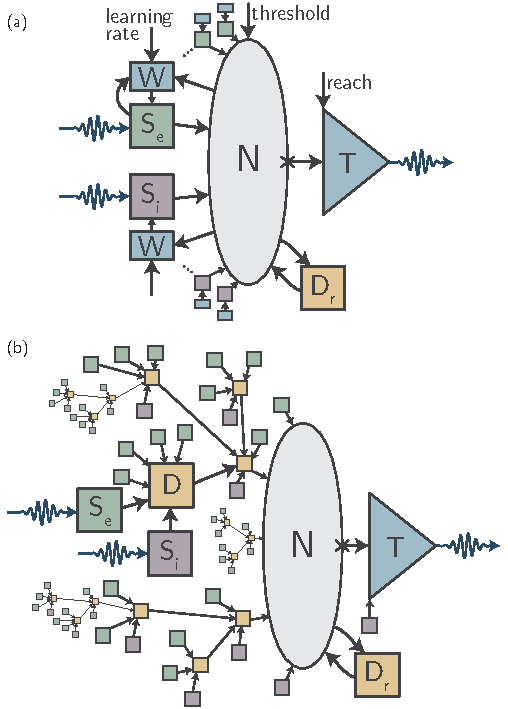
\includegraphics[width=8.6cm]{figures/_fig__schematics.pdf}
\captionof{figure}{\label{fig:schematic__circuits}Two schematics of loop neurons. (a) Schematic of point neuron. (b) Schematic of neuron with dendritic tree.}
\end{figure}

\begin{equation}
\label{eq:leaky_integrator}
\frac{dQ(t)}{dt} = f(t)-\frac{Q(t)}{\tau},
\end{equation}


\section{\label{sec:synapses}Synapses}


This description of the operation of the circuit is based on well-known properties of Josephson junctions within the formalism of the resistively and capacitively shunted junction (RCSJ) model \cite{vatu1998,ka1999,ti1996}. The relevant behavior derives from the fact that a JJ will produce a voltage fluxon after a time $t_{\mathrm{fq}}$ determined by the relation
\begin{equation}
\label{eq:jj__fluxon_production}
\int_0^{t_{\mathrm{fq}}}V(t)dt = \Phi_0.
\end{equation}
If $V(t)$ is slowly varying on the scale of $t^{\mathrm{fq}}$, we can make the approximation $V(t)\,t^{\mathrm{fq}} \approx \Phi_0$, giving the rate of fluxon generation as
\begin{equation}
\label{eq:jj__fluxon_rate}
R_{\mathrm{fq}}(t) =  \frac{1}{t_{\mathrm{fq}}} = \frac{V(t)}{\Phi_0}.
\end{equation}

\begin{equation}
\label{eq:synapses__leaky_integrator}
\frac{dI^{\mathrm{si}}(t)}{dt} = R_{\mathrm{fq}}\left(I^{\mathrm{sf}}(t),I^{\mathrm{si}}(t)\right)\,I_{\mathrm{fq}} -\frac{I^{\mathrm{si}}(t)}{\tau^{\mathrm{si}}},
\end{equation}
where the function $R^{\mathrm{fq}}\left(I^{\mathrm{sf}},I^{\mathrm{si}}\right)$ represents the rate at which fluxons are added to the SI loop as a function of the total current across the synaptic firing junction, $I^{\mathrm{sf}}$, as well the current circulating in the SI loop, $I^{\mathrm{si}}$. $I_{\mathrm{fq}} = \Phi_0/L^{\mathrm{si}}$ is the current added to the SI loop with each fluxon. The flux-induced current $I^{\mathrm{si}}$ circulates in the SI loop in a manner that counters the bias to $J^{\mathrm{si}}$. It is this counter-biasing that causes the SI loop to saturate as a function of $I^{\mathrm{si}}$. When $I^{\mathrm{si}}$ becomes sufficiently large, the fluxon generated by $J^{\mathrm{jtl}}$ does not provide enough current to drive $J^{\mathrm{si}}$ above $I_c$, and the stored flux in the SI loop must decay before subsequent synapse events can add to the integrated signal.

\begin{equation}
\label{eq:jj__current_voltage}
V^{\mathrm{sf}}(I^{\mathrm{sf}}) = \begin{cases} V_0\left[ \left( \frac{I^{\mathrm{sf}}}{I_c-I_r} \right)^{\mu_1} - 1 \right]^{\mu_2}, & \text{for } I > (I_c-I_r)_+ \\
0, & \text{for } I < (I_c)_-
\end{cases}
\end{equation} 
where the values $\mu_1$, $\mu_2$, and $V_0$ depend on the specific parameters of the shunt resistance and capacitance in the RCSJ model. For the junctions considered here, $I_r = 1.1768$\,\textmu A is the reset current associated with hysteresis on $J_{\mathrm{sf}}$ due to the fact that $\beta_c = 0.95 > 0$. $\mu_1 = 3.464271$, $\mu_2 = 0.306768$, and $V_0 = 233.966$\,\textmu V. From Eqs.\,\ref{eq:jj__fluxon_production} and \ref{eq:jj__current_voltage} we can obtain $r^{\mathrm{fq}}$. In the case where $I^{(\mathrm{sf})}$ is slowly varying compared to $t^fq$, $ r^{\mathrm{fq}} = V^{(\mathrm{sf})}/\Phi_0$. The notation $I > (I_c-I_r)_+$ refers to currents $I$ that have exceeded $I_c$, driving the junction into the resistive state, and have yet to drop below $I_c-I_r$, and are therefore demonstrating hysteresis. Likewise, $I<(I_c)_-$ refers to currents that are below $I_c$ while the junction is not in the hysteretic state.

To quantify the accuracy, we use a $\chi^2$ of the form
\begin{equation}
\label{eq:chi_squared}
\chi^2 = \frac{\int dt \left|I^{\mathrm{si}}_{\mathrm{spice}}(t) - I^{\mathrm{si}}_{\mathrm{ode}}(t)\right|^2}{\int dt \left|I^{\mathrm{si}}_{\mathrm{spice}}(t)\right|^2}.
\end{equation}

\begin{figure*}[h!]
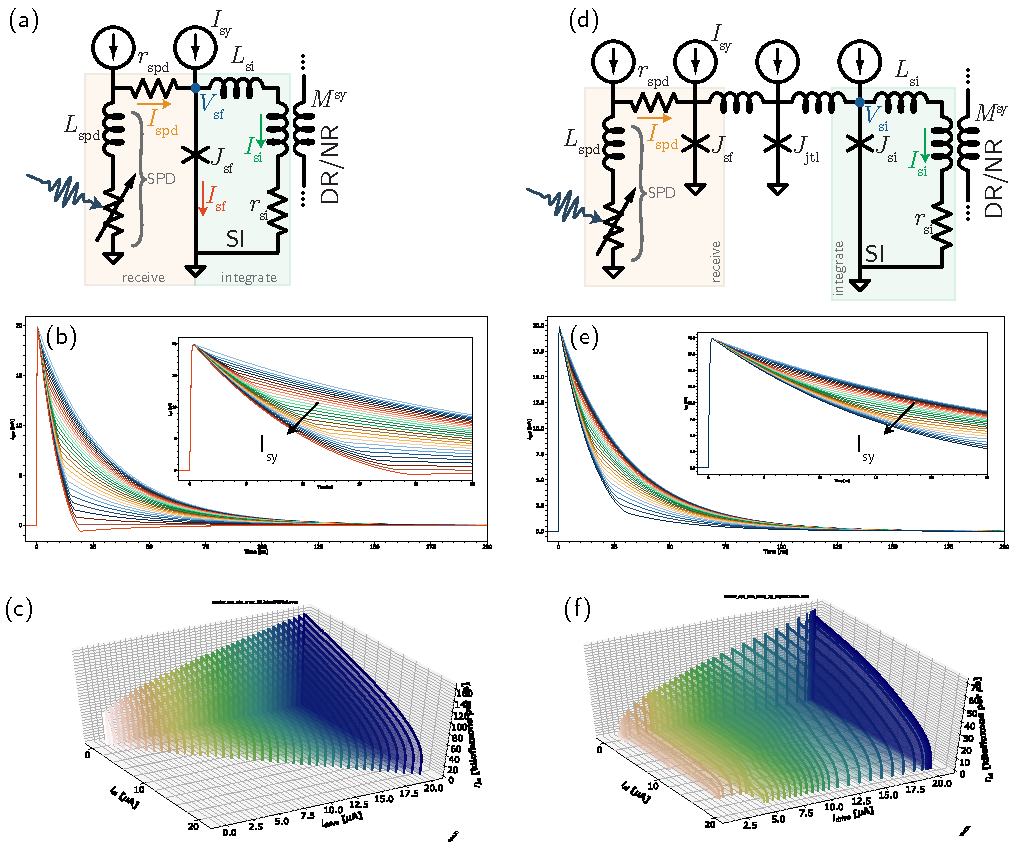
\includegraphics[width=17.2cm]{figures/_fig__synapses__circuits__responses.pdf}
\captionof{figure}{\label{fig:synapses__responses}Caption of fig:synapses circuitsresponses.}
\end{figure*}

\begin{figure*}[h!]
\includegraphics[width=17.2cm]{figures/_fig__synapses__comparison__1jj__tau_si.pdf}
\captionof{figure}{\label{fig:synapses__comparison__1jj__tau_si}Caption of fig:synapses comparison 1jj tau si.}
\end{figure*}

\begin{figure*}[h!]
\includegraphics[width=17.2cm]{figures/_fig__synapses__comparison__1jj__L_si.pdf}
\captionof{figure}{\label{fig:synapses__comparison__1jj__L_si}Caption of fig:synapses comparison 1jj L si.}
\end{figure*}

\begin{figure*}[h!]
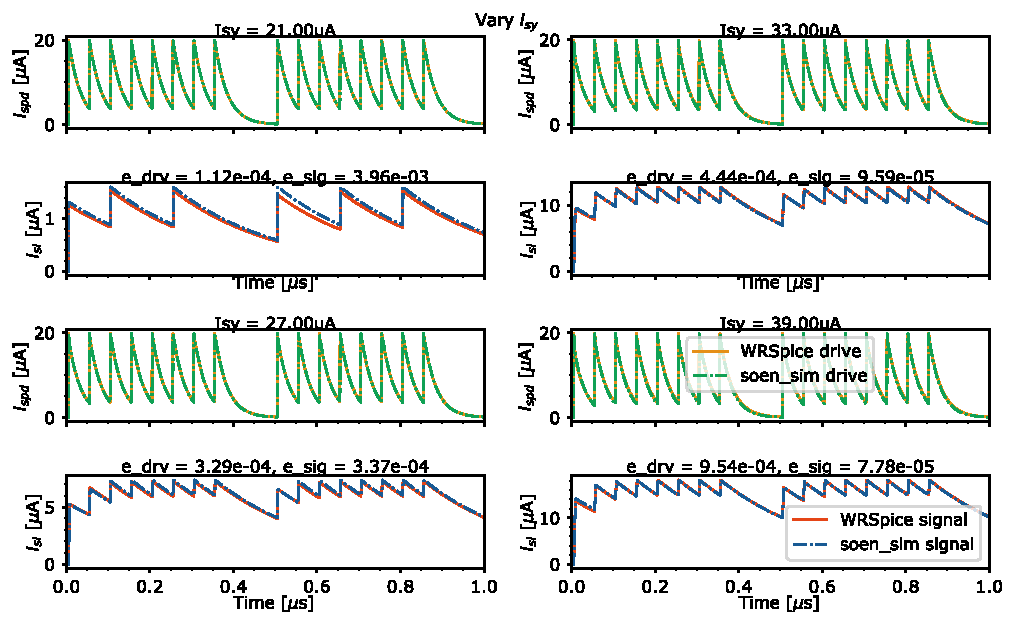
\includegraphics[width=17.2cm]{figures/_fig__synapses__comparison__1jj__I_sy.pdf}
\captionof{figure}{\label{fig:synapses__comparison__1jj__I_sy}Caption of fig:synapses comparison 1jj I sy.}
\end{figure*}

\begin{figure*}[h!]
\includegraphics[width=17.2cm]{figures/_fig__synapses__error_vs_dt__1jj.pdf}
\captionof{figure}{\label{fig:synapses__error_vs_dt__1jj}Caption of fig:synapses error vs dt 1jj.}
\end{figure*}

\begin{figure*}[h!]
\includegraphics[width=17.2cm]{figures/_fig__synapses__comparison__3jj__tau_si.pdf}
\captionof{figure}{\label{fig:synapses__comparison__3jj__tau_si}Caption of fig:synapses comparison 3jj tau si.}
\end{figure*}

\begin{figure*}[h!]
\includegraphics[width=17.2cm]{figures/_fig__synapses__comparison__3jj__L_si.pdf}
\captionof{figure}{\label{fig:synapses__comparison__3jj__L_si}Caption of fig:synapses comparison 3jj L si.}
\end{figure*}

\begin{figure*}[h!]
\includegraphics[width=17.2cm]{figures/_fig__synapses__comparison__3jj__I_sy.pdf}
\captionof{figure}{\label{fig:synapses__comparison__3jj__I_sy}Caption of fig:synapses comparison 3jj I sy.}
\end{figure*}

\begin{figure*}[h!]
\includegraphics[width=17.2cm]{figures/_fig__synapses__error_vs_dt__3jj.pdf}
\captionof{figure}{\label{fig:synapses__error_vs_dt__3jj}Caption of fig:synapses error vs dt 3jj.}
\end{figure*}

\section{\label{sec:dendrites}Dendrites}

\begin{equation}
\label{eq:dendrites__leaky_integrator}
\frac{dI^{\mathrm{di}}(t)}{dt} = R_{\mathrm{fq}} \left( \Phi^{\mathrm{dr}}_a(t),I^{\mathrm{di}}(t) \right)\,I_{\mathrm{fq}} - \frac{I^{\mathrm{di}}(t)}{\tau^{\mathrm{di}}}.
\end{equation}
$R_{\mathrm{fq}} \left( \Phi^{\mathrm{dr}}_a(t),I^{\mathrm{di}}(t) \right)$ is the rate function, and $\Phi^{\mathrm{dr}}_a(t)$ is the total applied flux to the dendritic receiving loop:
\begin{equation}
\label{eq:dendrites__applied_flux}
\Phi^{\mathrm{dr}}_a(t) = \sum_i M_i I_i^{\mathrm{si/di}}(t).
\end{equation}
The sum runs over all inputs to the dendritic receiving loop, and the superscript notation $I_i^{\mathrm{si/di}}$ indicates that inputs may be from synaptic or dendritic integration loops.

\begin{figure*}[h!]
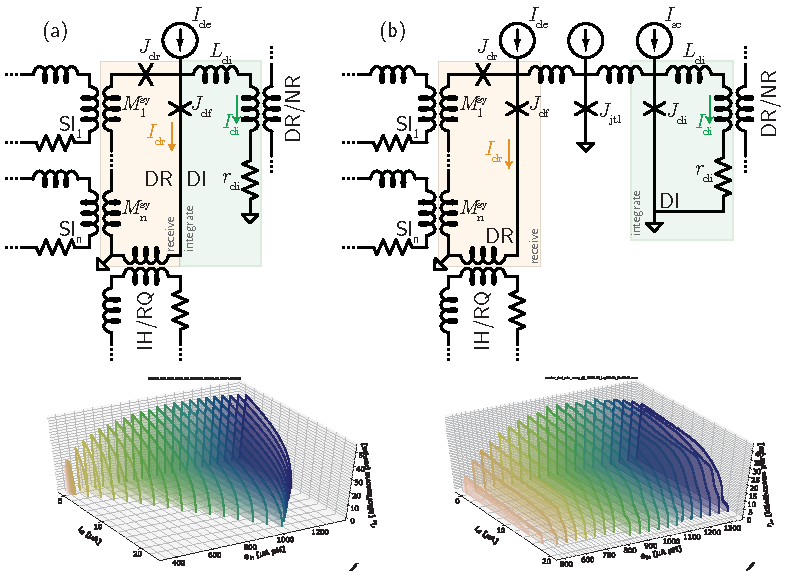
\includegraphics[width=17.2cm]{figures/_fig__dendrites__circuits__responses.pdf}
\captionof{figure}{\label{fig:dendrites__circuits__responses}Caption of fig:dendrites responses.}
\end{figure*}

\begin{figure}[h!]
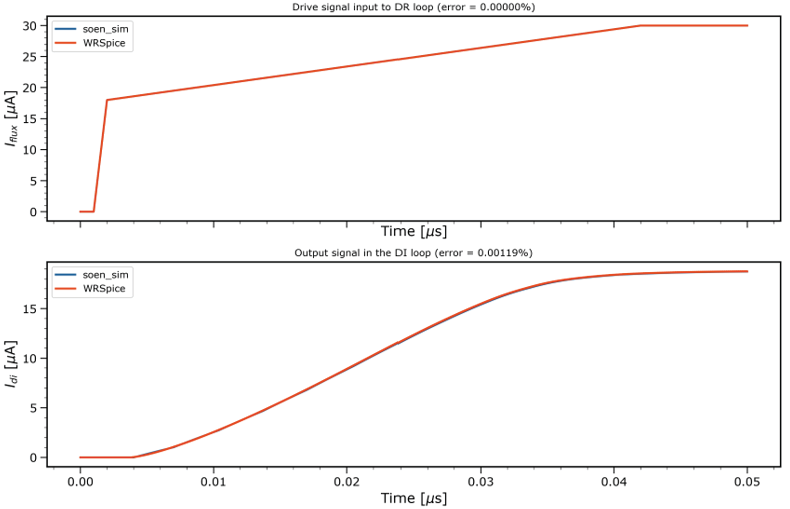
\includegraphics[width=8.6cm]{figures/_fig__dendrites__comparison__2jj__lin_ramp.pdf}
\captionof{figure}{\label{fig:dendrites__comparison__2jj__lin_ramp}Caption of fig:dendrites comparison 2jj lin ramp.}
\end{figure}

\begin{figure}[h!]
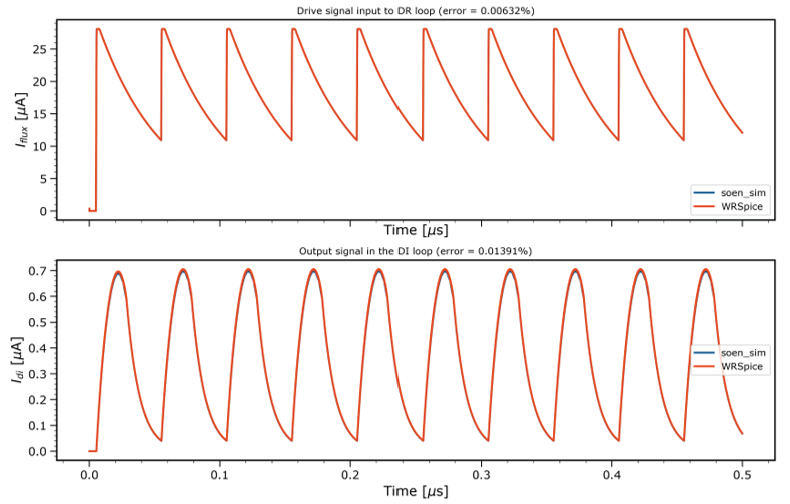
\includegraphics[width=8.6cm]{figures/_fig__dendrites__comparison__2jj__exp_pls_seq.pdf}
\captionof{figure}{\label{fig:dendrites__comparison__2jj__exp_pls_seq}Caption of fig:dendrites comparison exp pls seq.}
\end{figure}

\begin{figure}[h!]
\includegraphics[width=8.6cm]{figures/_fig__dendrites__comparison__2jj__sq_pls_seq.pdf}
\captionof{figure}{\label{fig:dendrites__comparison__2jj__sq_pls_seq}Caption of fig:dendrites comparison sq pls seq.}
\end{figure}

\begin{figure}[h!]
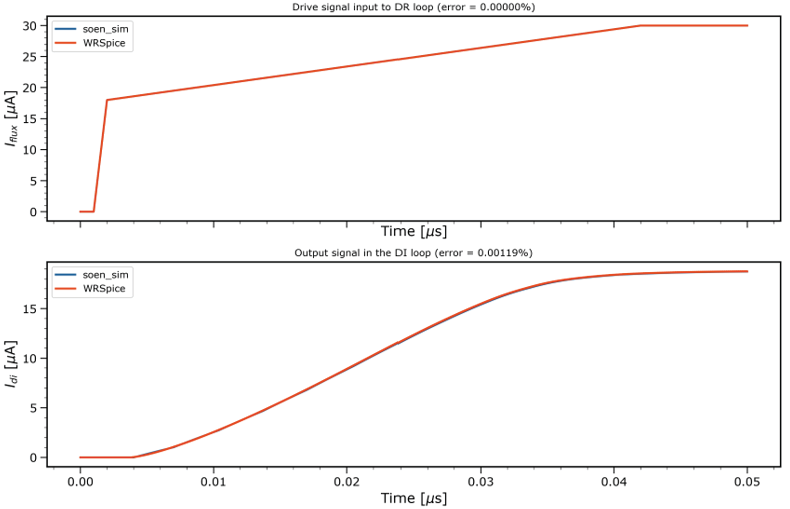
\includegraphics[width=8.6cm]{figures/_fig__dendrites__comparison__4jj__lin_ramp.pdf}
\captionof{figure}{\label{fig:dendrites__comparison__4jj__lin_ramp}Caption of fig:dendrites comparison 4jj lin ramp.}
\end{figure}

\begin{figure}[h!]
\includegraphics[width=8.6cm]{figures/_fig__dendrites__comparison__4jj__sq_pls_seq.pdf}
\captionof{figure}{\label{fig:dendrites__comparison__4jj__sq_pls_seq}Caption of fig:dendrites comparison 4jj sq pls seq.}
\end{figure}

\begin{figure}[h!]
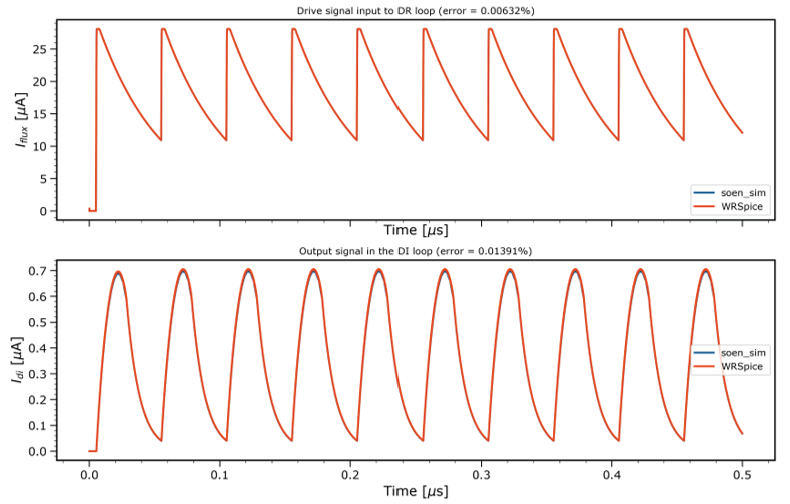
\includegraphics[width=8.6cm]{figures/_fig__dendrites__comparison__4jj__exp_pls_seq.pdf}
\captionof{figure}{\label{fig:dendrites__comparison__4jj__exp_pls_seq}Caption of fig:dendrites comparison 4jj exp pls seq.}
\end{figure}

\begin{figure}[h!]
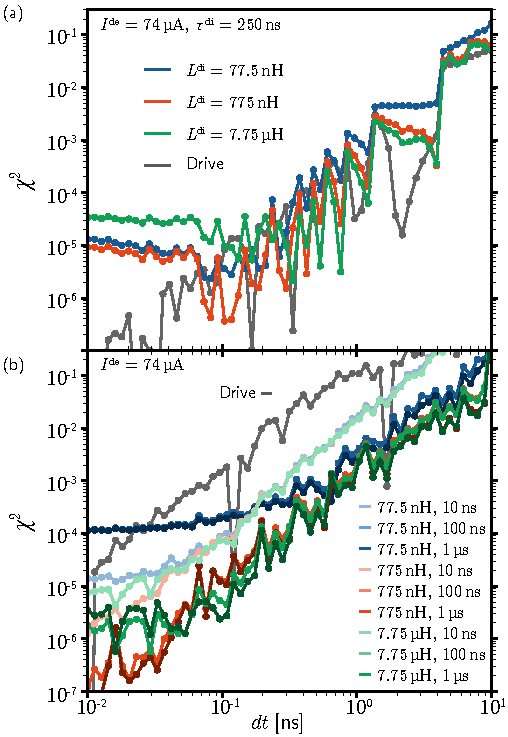
\includegraphics[width=8.6cm]{figures/_fig__dendrites__error_vs_dt__2jj.pdf}
\captionof{figure}{\label{fig:dendrites__error_vs_dt__2jj}Caption of fig:dendrites 2jj error vs dt.}
\end{figure}

\begin{figure}[h!]
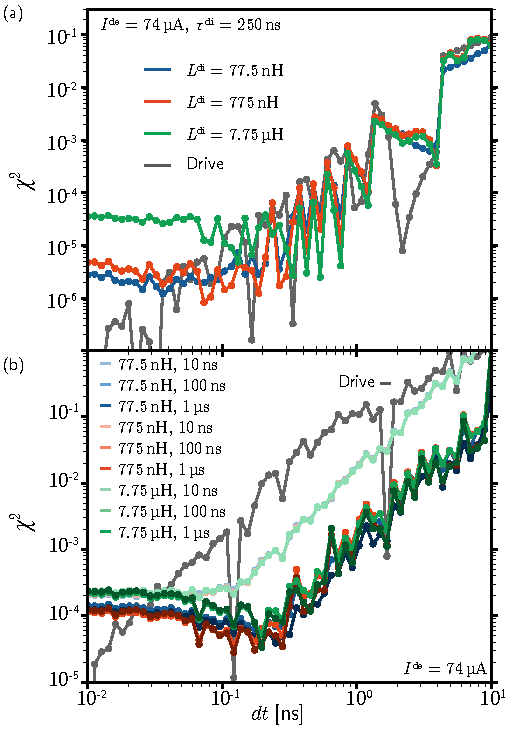
\includegraphics[width=8.6cm]{figures/_fig__dendrites__error_vs_dt__4jj.pdf}
\captionof{figure}{\label{fig:dendrites__error_vs_dt__4jj}Caption of fig:dendrites 4jj error vs dt.}
\end{figure}

\section{\label{sec:neurons}Neurons}

\begin{figure}[h!]
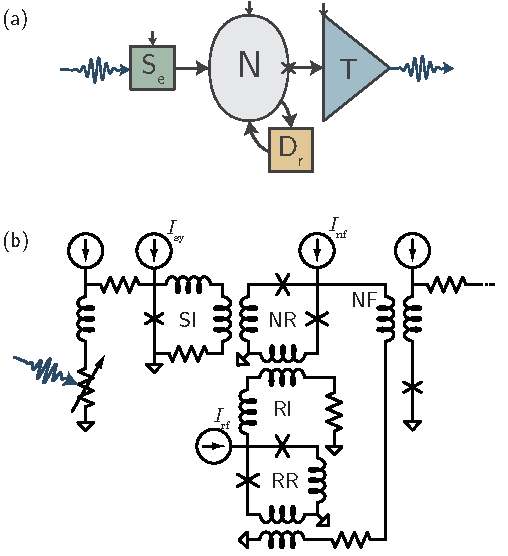
\includegraphics[width=8.6cm]{figures/_fig__point_neuron__one_synapse__schematic__circuit.pdf}
\captionof{figure}{\label{fig:point_neuron__one_synapse__schematic__circuit}Caption of fig:point neuron  one synapse  schematic  circuit.}
\end{figure}

\begin{figure*}[h!]
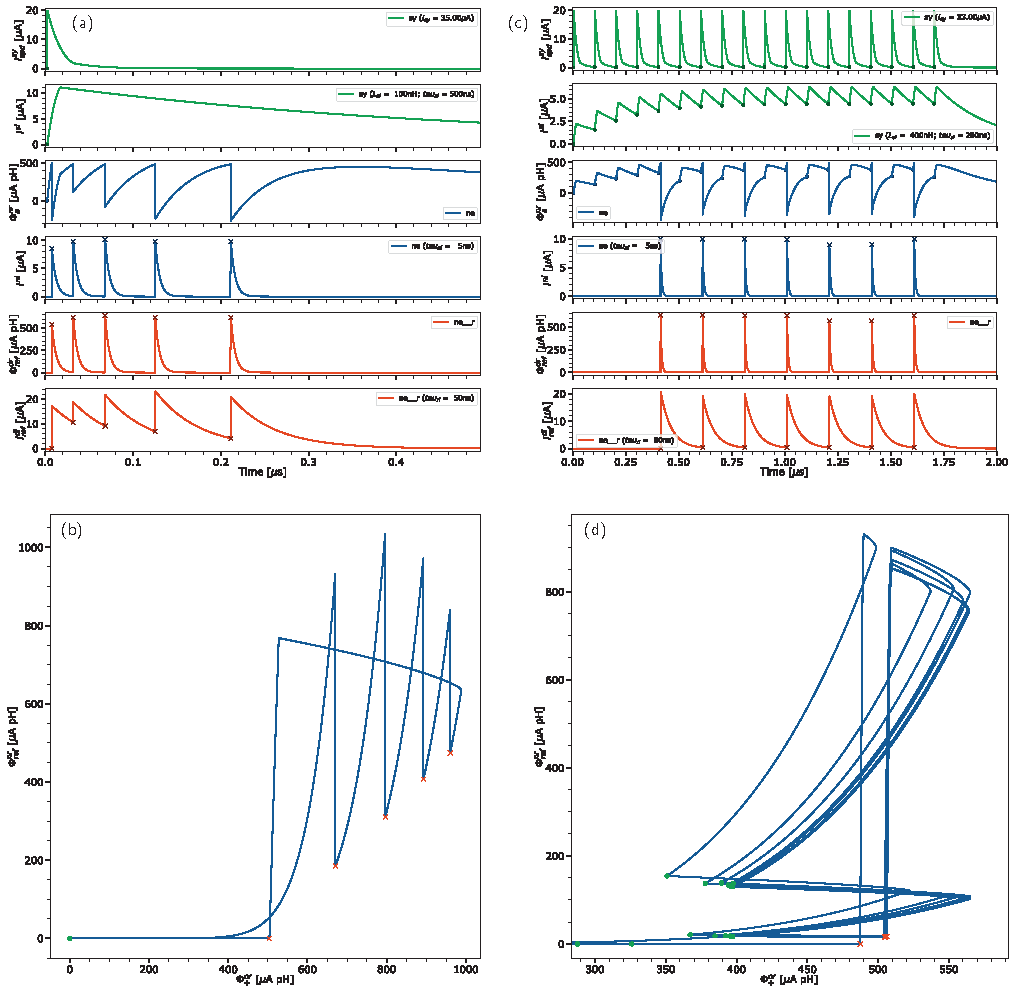
\includegraphics[width=17.2cm]{figures/_fig__point_neuron__one_synapse__data.pdf}
\captionof{figure}{\label{fig:point_neuron__one_synapse__data}Caption of fig:point neuron  one synapse  data.}
\end{figure*}

\begin{figure}[h!]
\includegraphics[width=8.6cm]{figures/_fig__point_neuron__nine_synapses__schematic.pdf}
\captionof{figure}{\label{fig:point_neuron__nine_synapses__schematic__circuit}Caption of fig:point neuron  nine  synapses  schematic.}
\end{figure}

\begin{figure*}[h!]

\includegraphics[width=17.2cm]{figures/_fig__point_neuron__nine_synapses__data.pdf}
\captionof{figure}{\label{fig:point_neuron__nine_synapses__data}Caption of fig:point neuron  nine synapses  data.}
\end{figure*}

\section{\label{sec:discussion}Discussion}

\vspace{1em}
\section{\label{sec:acknowledgements}Acknowledgements}
\noindent This is a contribution of NIST, an agency of the US government, not subject to copyright.

\appendix

\section{\label{apx:synapses}Further data regarding synapse modeling}

\section{\label{apx:dendrites}Further data regarding dendrite modeling}

\begin{figure}[h!]
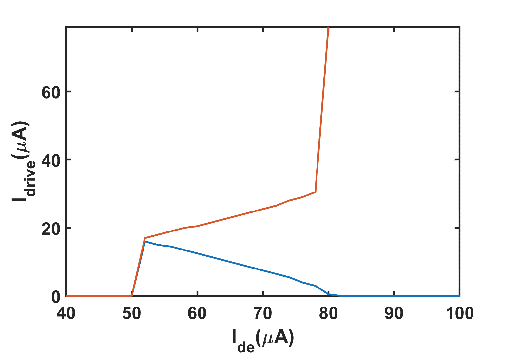
\includegraphics[width=8.6cm]{figures/_fig__dendrites__min_max__2jj.pdf}
\captionof{figure}{\label{fig:dendrites_min_max__2jj}Caption of fig:dendrites min max 2jj.}
\end{figure}

\begin{figure}[h!]
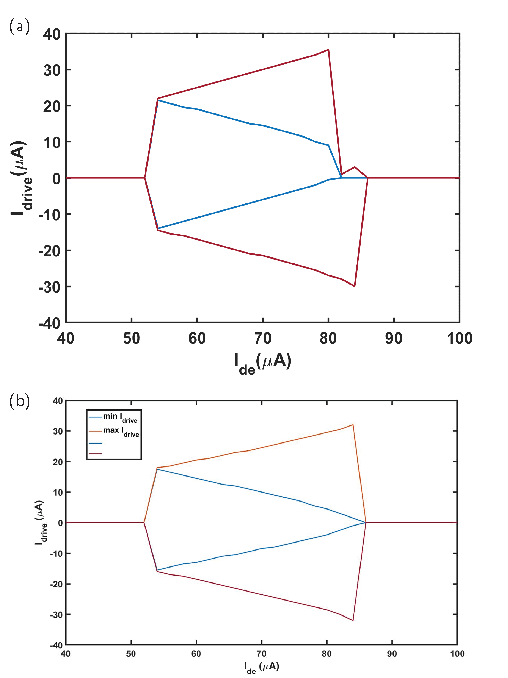
\includegraphics[width=8.6cm]{figures/_fig__dendrites__min_max__4jj.pdf}
\captionof{figure}{\label{fig:dendrites_min_max__4jj}Caption of fig:dendrites min max 4jj.}
\end{figure}

\section{\label{apx:fan_in}Analysis of dendritic and neuronal fan-in}

\begin{figure}[h!]
\includegraphics[width=8.6cm]{figures/_fig__fan-in__circuits.pdf}
\captionof{figure}{\label{fig:fan-in__circuits}Caption of fig:fan-in circuits.}
\end{figure}

We would like to know how to choose the inductors shown in Fig.\,\ref{fig:fan-in__circuits}(a) so the applied flux stays in the appropriate operating range as the number of synaptic connections, $N$, is modified. This consideration will identify the limit of how many synapses can be coupled to a single dendrite or neuron\textemdash the fan-in limit. 

We have seen that the operation of a dendrite (or neuron cell body) is significantly shaped by the inductance of the DR loop. We would therefore like to be able to increase the number of synaptic connections without changing the total inductance of this loop. This total inductance is given by
\begin{equation}
\label{eq:fan-in__direct_input__si_inductance}
L^{\mathrm{nr1}}_{\mathrm{tot}} = \sum_i L^{\mathrm{nr1}}_i = N L^{\mathrm{nr1}}_0
\end{equation}
We would like $L^{\mathrm{nr1}}_{\mathrm{tot}}$ to be independent of $N$, which is possible with $L^{\mathrm{nr1}}_N = L^{\mathrm{nr1}}_0/N$. The total applied flux to the NR loop is given by
\begin{equation}
\label{eq:fan-in__direct_input__applied_flux}
\Phi_{\mathrm{a}}^{\mathrm{nr}} = \sum_i M_i^{\mathrm{si|nr}} \, I_i^{\mathrm{si}}.
\end{equation}
Suppose all SI loops contain a given current, $I_0^{\mathrm{si}}$. We would like the applied flux to the NR loop, $\Phi_{\mathrm{a}}^{\mathrm{nr}}$, to be independent of $N$:
\begin{equation}
\label{eq:fan-in__direct_input__flux_independent_of_N}
\frac{ \Phi_{\mathrm{a}}^{\mathrm{nr}} }{ I_0^{\mathrm{si}} } = \mathrm{cnst.} \neq f(N).
\end{equation}
In the case where all mutual inductors between synapses and the NR loop are equal,
\begin{equation}
\label{eq:fan-in__direct_input__flux_independent_of_N_2}
\frac{ \Phi_{\mathrm{a}}^{\mathrm{nr}}(N) }{ I_0^{\mathrm{si}} } = N\,k\,\sqrt{ L_N^{\mathrm{si2}} \, L_N^{\mathrm{nr1}}},
\end{equation}
where $L_N^{\mathrm{si2}}$ and $L_N^{\mathrm{nr1}}$ are the value ofs $L^{\mathrm{si2}}$ and $L^{\mathrm{nr1}}$ that we should choose for the SI loop output inductor when there are $N$ synapses coupled directly to the NR loop. We have seen above that we need $L_N^{\mathrm{nr1}} = L_0^{\mathrm{nr1}}/N$ to maintain the inductance of the NR loop. Therefore, in order for Eq.\,\ref{eq:fan-in__direct_input__flux_independent_of_N_2} to satisfy Eq.\,\ref{eq:fan-in__direct_input__flux_independent_of_N}, we must also have $L_N^{\mathrm{si2}} = L_0^{\mathrm{si2}}/N$.

This consideration does not explicitly identify a fan-in limit. This limit arises due to practical considerations related to making $L^{\mathtrm{si2}}$ and $L^{\mathtrm{nr1}}$ exceedingly small as $N$ grows large. With $L_0 \approx 1$\,pH a rough lower limit on what we would like to fabricate, and $L_{\mathrm{tot}}^{\mathrm{nr}} \approx 20$\,pH, we see direct fan-in with this circuit design is limited to about 20. This limit can be straightforwardly overcome with an intermediate transformer collection coil, as shown in Fig.\,\ref{fig:fan-in__circuits}(b).

\begin{equation}
\label{eq:fan-in__transformer_collection}
\frac{\Phi_{\mathrm{a}}^{\mathrm{nr}}}{I_0^\mathrm{si}} \approx \frac{ M^{\mathrm{si|nt}} \, M^{\mathrm{nt|nr}} }{L^{\mathrm{nt1}}} \left( 1-\epsilon \right) + \mathcal{O}(\epsilon^2)
\end{equation}
$M^{\mathrm{si|nt}} = k\sqrt{L^{\mathrm{si2}} \, L^{\mathrm{nt1}}}$ and $M^{\mathrm{nt|nr}} = k\sqrt{L^{\mathrm{nt3}} \, L^{\mathrm{nr1}}}$

\begin{equation}
\label{eq:fan-in__transformer_collection__epsilon}
\epsilon \equiv \frac{ L^{\mathrm{nt2}}+L^{\mathrm{nt3}} }{ N L^{\mathrm{nt1}} }
\end{equation}


\bibliographystyle{unsrt}
\bibliography{phenomenological_modeling}

\end{document}